% Options for packages loaded elsewhere
% Options for packages loaded elsewhere
\PassOptionsToPackage{unicode}{hyperref}
\PassOptionsToPackage{hyphens}{url}
\PassOptionsToPackage{dvipsnames,svgnames,x11names}{xcolor}
%
\documentclass[
  11pt,
  a4paper,
]{article}
\usepackage{xcolor}
\usepackage[margin=25mm]{geometry}
\usepackage{amsmath,amssymb}
\setcounter{secnumdepth}{-\maxdimen} % remove section numbering
\usepackage{iftex}
\ifPDFTeX
  \usepackage[T1]{fontenc}
  \usepackage[utf8]{inputenc}
  \usepackage{textcomp} % provide euro and other symbols
\else % if luatex or xetex
  \usepackage{unicode-math} % this also loads fontspec
  \defaultfontfeatures{Scale=MatchLowercase}
  \defaultfontfeatures[\rmfamily]{Ligatures=TeX,Scale=1}
\fi
\usepackage{lmodern}
\ifPDFTeX\else
  % xetex/luatex font selection
\fi
% Use upquote if available, for straight quotes in verbatim environments
\IfFileExists{upquote.sty}{\usepackage{upquote}}{}
\IfFileExists{microtype.sty}{% use microtype if available
  \usepackage[]{microtype}
  \UseMicrotypeSet[protrusion]{basicmath} % disable protrusion for tt fonts
}{}
\makeatletter
\@ifundefined{KOMAClassName}{% if non-KOMA class
  \IfFileExists{parskip.sty}{%
    \usepackage{parskip}
  }{% else
    \setlength{\parindent}{0pt}
    \setlength{\parskip}{6pt plus 2pt minus 1pt}}
}{% if KOMA class
  \KOMAoptions{parskip=half}}
\makeatother
% Make \paragraph and \subparagraph free-standing
\makeatletter
\ifx\paragraph\undefined\else
  \let\oldparagraph\paragraph
  \renewcommand{\paragraph}{
    \@ifstar
      \xxxParagraphStar
      \xxxParagraphNoStar
  }
  \newcommand{\xxxParagraphStar}[1]{\oldparagraph*{#1}\mbox{}}
  \newcommand{\xxxParagraphNoStar}[1]{\oldparagraph{#1}\mbox{}}
\fi
\ifx\subparagraph\undefined\else
  \let\oldsubparagraph\subparagraph
  \renewcommand{\subparagraph}{
    \@ifstar
      \xxxSubParagraphStar
      \xxxSubParagraphNoStar
  }
  \newcommand{\xxxSubParagraphStar}[1]{\oldsubparagraph*{#1}\mbox{}}
  \newcommand{\xxxSubParagraphNoStar}[1]{\oldsubparagraph{#1}\mbox{}}
\fi
\makeatother


\usepackage{longtable,booktabs,array}
\newcounter{none} % for unnumbered tables
\usepackage{calc} % for calculating minipage widths
% Correct order of tables after \paragraph or \subparagraph
\usepackage{etoolbox}
\makeatletter
\patchcmd\longtable{\par}{\if@noskipsec\mbox{}\fi\par}{}{}
\makeatother
% Allow footnotes in longtable head/foot
\IfFileExists{footnotehyper.sty}{\usepackage{footnotehyper}}{\usepackage{footnote}}
\makesavenoteenv{longtable}
\usepackage{graphicx}
\makeatletter
\newsavebox\pandoc@box
\newcommand*\pandocbounded[1]{% scales image to fit in text height/width
  \sbox\pandoc@box{#1}%
  \Gscale@div\@tempa{\textheight}{\dimexpr\ht\pandoc@box+\dp\pandoc@box\relax}%
  \Gscale@div\@tempb{\linewidth}{\wd\pandoc@box}%
  \ifdim\@tempb\p@<\@tempa\p@\let\@tempa\@tempb\fi% select the smaller of both
  \ifdim\@tempa\p@<\p@\scalebox{\@tempa}{\usebox\pandoc@box}%
  \else\usebox{\pandoc@box}%
  \fi%
}
% Set default figure placement to htbp
\def\fps@figure{htbp}
\makeatother


% definitions for citeproc citations
\NewDocumentCommand\citeproctext{}{}
\NewDocumentCommand\citeproc{mm}{%
  \begingroup\def\citeproctext{#2}\cite{#1}\endgroup}
\makeatletter
 % allow citations to break across lines
 \let\@cite@ofmt\@firstofone
 % avoid brackets around text for \cite:
 \def\@biblabel#1{}
 \def\@cite#1#2{{#1\if@tempswa , #2\fi}}
\makeatother
\newlength{\cslhangindent}
\setlength{\cslhangindent}{1.5em}
\newlength{\csllabelwidth}
\setlength{\csllabelwidth}{3em}
\newenvironment{CSLReferences}[2] % #1 hanging-indent, #2 entry-spacing
 {\begin{list}{}{%
  \setlength{\itemindent}{0pt}
  \setlength{\leftmargin}{0pt}
  \setlength{\parsep}{0pt}
  % turn on hanging indent if param 1 is 1
  \ifodd #1
   \setlength{\leftmargin}{\cslhangindent}
   \setlength{\itemindent}{-1\cslhangindent}
  \fi
  % set entry spacing
  \setlength{\itemsep}{#2\baselineskip}}}
 {\end{list}}
\usepackage{calc}
\newcommand{\CSLBlock}[1]{\hfill\break\parbox[t]{\linewidth}{\strut\ignorespaces#1\strut}}
\newcommand{\CSLLeftMargin}[1]{\parbox[t]{\csllabelwidth}{\strut#1\strut}}
\newcommand{\CSLRightInline}[1]{\parbox[t]{\linewidth - \csllabelwidth}{\strut#1\strut}}
\newcommand{\CSLIndent}[1]{\hspace{\cslhangindent}#1}



\setlength{\emergencystretch}{3em} % prevent overfull lines

\providecommand{\tightlist}{%
  \setlength{\itemsep}{0pt}\setlength{\parskip}{0pt}}



 


\usepackage{booktabs}
\usepackage{longtable}
\usepackage{array}
\usepackage{multirow}
\usepackage{wrapfig}
\usepackage{float}
\usepackage{colortbl}
\usepackage{pdflscape}
\usepackage{tabu}
\usepackage{threeparttable}
\usepackage{threeparttablex}
\usepackage[normalem]{ulem}
\usepackage{makecell}
\usepackage{xcolor}
\renewcommand{\baselinestretch}{1.1}
\usepackage{microtype}
\frenchspacing
\renewcommand{\baselinestretch}{1.1}
\usepackage{graphicx}
\usepackage{xcolor}
\usepackage{amsmath,amssymb}
\usepackage{booktabs}
\usepackage{longtable}
\usepackage{array}
\usepackage{multirow}
\usepackage{makecell}
\usepackage{pdflscape}
\usepackage{float}
\usepackage{fancyhdr}
\makeatletter
\@ifpackageloaded{caption}{}{\usepackage{caption}}
\AtBeginDocument{%
\ifdefined\contentsname
  \renewcommand*\contentsname{Table of contents}
\else
  \newcommand\contentsname{Table of contents}
\fi
\ifdefined\listfigurename
  \renewcommand*\listfigurename{List of Figures}
\else
  \newcommand\listfigurename{List of Figures}
\fi
\ifdefined\listtablename
  \renewcommand*\listtablename{List of Tables}
\else
  \newcommand\listtablename{List of Tables}
\fi
\ifdefined\figurename
  \renewcommand*\figurename{Figure}
\else
  \newcommand\figurename{Figure}
\fi
\ifdefined\tablename
  \renewcommand*\tablename{Table}
\else
  \newcommand\tablename{Table}
\fi
}
\@ifpackageloaded{float}{}{\usepackage{float}}
\floatstyle{ruled}
\@ifundefined{c@chapter}{\newfloat{codelisting}{h}{lop}}{\newfloat{codelisting}{h}{lop}[chapter]}
\floatname{codelisting}{Listing}
\newcommand*\listoflistings{\listof{codelisting}{List of Listings}}
\makeatother
\makeatletter
\makeatother
\makeatletter
\@ifpackageloaded{caption}{}{\usepackage{caption}}
\@ifpackageloaded{subcaption}{}{\usepackage{subcaption}}
\makeatother
\usepackage{bookmark}
\IfFileExists{xurl.sty}{\usepackage{xurl}}{} % add URL line breaks if available
\urlstyle{same}
\hypersetup{
  pdftitle={Tree Based Decomposition of Health Inequalities},
  pdfauthor={Moses Mburu (2469245)},
  colorlinks=true,
  linkcolor={blue},
  filecolor={Maroon},
  citecolor={Blue},
  urlcolor={Blue},
  pdfcreator={LaTeX via pandoc}}


\title{Tree Based Decomposition of Health Inequalities}
\author{Moses Mburu (2469245)}
\date{}
\begin{document}
\maketitle


\section{Introduction}\label{sec-introduction}

Child survival has improved since 1990, but the gains have not closed
the gap between countries or between groups of children. Globally,
under-five mortality fell from 93 deaths per 1,000 live births in 1990
to 37.7 in 2019, and the number of under-five deaths fell from 12.5
million to 5.2 million
(\citeproc{ref-sharrow2022_under5_mortality}{{Sharrow \emph{et al.}},
2022}). Reduction in under-5 mortality are linked to improved child
health services, greater access to care, and lower levels of extreme
poverty (\citeproc{ref-jones2003_child_survival}{Jones \emph{et al.},
2003}). The burden, however, is still concentrated in poorer settings.
The latest (\citeproc{ref-who_gho_under5_mortality_indicator}{World
Health Organisation, 2026}) estimates show that sub-Saharan Africa had
the highest regional under-five mortality rate, 67 per 1000 live births,
and almost half of all under-five deaths occurred in five countries,
including the Democratic Republic of the Congo
(\citeproc{ref-sharrow2022_under5_mortality}{{Sharrow \emph{et al.}},
2022}). Within these countries, a child's risk also depends on household
poverty, proximity to health services, access to clean water,
sanitation, and health information, and place of residence. Even a
better-off household may remain at risk when local services are weak or
far away. For this reason, studying socioeconomic inequality in
under-five mortality helps show which children are still exposed to
risks that can be prevented.

When statistical methods such as regression analysis are used in policy
making, a national estimate may show that poorer children have higher
mortality rates. However, it can hide subgroup differences linked to
household conditions, province(administrative areas), maternal
background, or demographic characteristics. Identifying risk groups
matters because interventions are organised in real settings, through
health facilities, communities, provinces(administrative areas), and
programme catchment areas. A more detailed inequality analysis can
therefore identify the groups that should receive attention and indicate
where a single public health response may not be sufficient.

Health inequality analysis commonly begins by ordering individuals or
households according to socioeconomic position and then examining how
the health outcome is distributed along that ordering. The concentration
index provides a standard way to summarise this relationship
(\citeproc{ref-wagstaff2003decomposing}{{Wagstaff, van Doorslaer and
Watanabe}, 2003}). Classical decomposition methods then use a regression
model to estimate how different determinants contribute to the observed
inequality in the outcome
(\citeproc{ref-wagstaff2003decomposing}{{Wagstaff, van Doorslaer and
Watanabe}, 2003}; \citeproc{ref-speybroeck2010decomposing}{Speybroeck
\emph{et al.}, 2010}). This is useful because it gives a direct additive
breakdown. At the same time, the interpretation depends on the average
effects from the fitted model. An important structure can therefore be
missed if mortality risk varies across subgroups, if determinants act
jointly, or if the relationship differs above and below certain
thresholds.

In this thesis, we develop a tree-based way of decomposing socioeconomic
inequality in health. The method still uses the concentration index, but
places it inside the splitting process of a tree. A typical decision
tree chooses a split because it improves predictive performance. Here,
the split is chosen because it separates the data into groups where
socioeconomic inequality in the outcome is lower within each group. The
fitted tree then produces decision rules that describe population
groups. These rules are easier to discuss in public health work than
regression coefficients alone, because they point to groups that policy
makers, programme teams, and public health planners can recognise and
act on.

At each node, the tree searches across candidate variables and
admissible split points, then selects the variable and split pair that
gives the largest reduction in weighted within-node concentration-index
impurity. The fitted tree is stored using the partykit tree
representation for plotting and traversal
(\citeproc{ref-hothorn2015partykit}{Hothorn and Zeileis, 2015}), but the
tree-growing rule is not the conditional-inference variable-selection
rule. We then apply the same split logic in a random forest setting. The
forest is useful because it averages many inequality-oriented trees and
is less dependent on any single early split, although this also makes
the fitted structure less transparent. To recover a readable summary of
the forest, we fit a surrogate tree to the forest predictions. This
follows the idea of using a representative tree to summarise the main
behaviour of an ensemble in a form that can be read as decision rules
(\citeproc{ref-banerjee2012representative_trees}{Banerjee, Ding and
Noone, 2012}). Finally, we use SHAP values to express the fitted
tree-based predictions as additive feature contributions
(\citeproc{ref-lundberg2017unified}{Lundberg and Lee, 2017};
\citeproc{ref-lundberg2018tree}{Lundberg, Erion and Lee, 2018}). The
surrogate tree summarises the main subgroup structure, while SHAP
provides contributions at the level of the determinants.

For the analysis, we use child-level data from the Democratic Republic
of the Congo DHS phase 8 survey
(\citeproc{ref-dhs_drc_2023_24_dataset}{The DHS Program, 2024}).
Under-five mortality is treated as the outcome, and the DHS household
wealth index serves as the socioeconomic ranking variable. This is
appropriate for the DRC setting, where DHS-based research has shown that
poverty and education are associated with access to health insurance
(\citeproc{ref-tsala_dimbuene2022_drc_health_insurance}{Tsala Dimbuene,
Muanza Nzuzi and Nzita Kikhela, 2022}). The splitting variables cover
characteristics of the child, the mother, the household, occupation,
residence, and province.

The thesis is organised around four objectives. The first is to define
the concentration index and demonstrate how it can serve as a splitting
criterion in recursive partitioning. The second is to apply
concentration-index trees and forests to under-five mortality using the
DRC DHS data. The third is to examine whether different
concentration-based impurity measures yield distinct split choices. The
fourth is to use SHAP-based contributions to decompose the concentration
index of the fitted tree-based predictions.

\section{Methodology}\label{sec-methodology}

\subsection{1. Data, Outcome, and
Determinants}\label{sec-data-outcome-determinants}

This thesis uses child-level data from the Democratic Republic of the
Congo DHS Phase 8 survey (\citeproc{ref-dhs_drc_2023_24_dataset}{The DHS
Program, 2024}). The analysis includes children with complete
information on the outcome, household wealth score, survey weight, and
covariates used in the tree models. DHS sampling weights are rescaled
and used as non-negative case weights in the inequality-tree fitting
procedure.

The outcome is under-five mortality, a binary adverse outcome:

\[
Y_i =
\begin{cases}
1, & \text{if child } i \text{ died before 60 months of age},\\
0, & \text{otherwise}.
\end{cases}
\]

The coding uses the child's survival status and age at death. Children
who died before 60 months receive a value of one. Since the outcome is
adverse, higher fitted values correspond to higher mortality risk.

Socioeconomic position is measured using the DHS household wealth index.
The continuous wealth score is used to rank children from poorer to
richer households when computing the concentration index. Wealth defines
the socioeconomic scale along which mortality inequality is measured.

The independent variables describe the child, mother, household,
occupation, residence, and province. They include child sex, birth-order
and birth-interval group, mother's age group, rural residence, mother's
and partner's education, mother's and partner's occupation, whether
either parent belongs to a low-skill or non-working occupational group,
and province. Categorical variables are recoded into interpretable
groups before the tree is fitted.

\subsection{2. Measuring Socioeconomic Inequality in
Health}\label{sec-measuring-socioeconomic-inequality}

This methodology aims to develop a decomposition of health inequalities
using tree methods. We will first introduce the concepts of health
inequality decomposition, then move to tree-based methods.

\subsubsection{2.1 The Concentration
Index}\label{sec-concentration-index}

The concentration index measures socioeconomic-related inequality in a
health variable. It uses the concentration curve, which plots the
cumulative proportion of the health variable on the vertical axis
against the cumulative proportion of the population on the horizontal
axis. Individuals are ordered from the most disadvantaged to the most
advantaged before constructing the curve
(\citeproc{ref-wagstaff2003decomposing}{{Wagstaff, van Doorslaer and
Watanabe}, 2003}). When the curve follows the 45-degree line, the health
variable has the same distribution across the socioeconomic ranking.

\(y_i\) denotes the health variable for individual \(i\), and let
\(R_i\) denote that individual's fractional socioeconomic rank, ordered
from poorest to richest. For an unweighted sample, the fractional rank
is

\[
R_i = \frac{i - 0.5}{n},
\]

where \(i = 1, \dots, n\) denotes the individual's position in the
socioeconomic ranking. If \(\mu\) is the mean of \(y\), the
concentration index is

\[
C = \frac{2}{n\mu}\sum_{i=1}^{n} y_i R_i - 1.
\]

A value of zero indicates no socioeconomic-related inequality in the
health variable. A negative value indicates that the variable is
concentrated among poorer individuals, while a positive value indicates
that it is concentrated among richer individuals. The sign, therefore,
depends on the meaning of the health variable. For adverse outcomes such
as mortality, illness, or malnutrition, a negative concentration index
indicates inequality that disadvantages people with low incomes.

In the simulated example in Figure~\ref{fig-concentration-curve}, we
simulate the health outcome to be concentrated among poorer individuals,
so the curve lies above the 45-degree line and the concentration index
is negative (-0.314).

\begin{figure}[H]

\centering{

\pandocbounded{
\includegraphics[keepaspectratio]{methodology_files/figure-pdf/fig-concentration-curve-1.pdf}}

}

\caption{\label{fig-concentration-curve}Illustration of a concentration
curve using a simple hypothetical example.}

\end{figure}%

\subsubsection{2.2 Decomposing Socioeconomic Inequality in
Health}\label{sec-decomposing-inequality}

Inequality is measured in the observed health outcome \(y_i\), but
interventions usually work through the factors that affect health rather
than through the outcome itself. Decomposition helps relate inequality
in \(y_i\) to the observed social determinants that may explain it.

Let the health outcome for the individual \(i\) be defined.

\[
y_i = f(x_i) + \varepsilon_i,
\]

where \(x_i\) denotes the observed determinants and \(\varepsilon_i\)
represents the part that the model does not explain. Let
\(\hat{y}_i = f(x_i)\) be the fitted value, and use this fitted model to
decompose the concentration index. \[
C = \frac{2}{n\mu}\sum_{i=1}^{n} \hat{y}_i R_i - 1,
\]

where:

\(\hat{y}_i\) is the estimated health outcome for an individual \(i\)
based on the observed determinants \(x_i\).
(\citeproc{ref-wagstaff2003decomposing}{{Wagstaff, van Doorslaer and
Watanabe}, 2003}) showed that the decomposition of the concentration
index results in the following expressions: \[
C = \sum_k \left( \frac{\beta_k \bar{x}_k}{\mu} \right) C_k + \frac{GC_\varepsilon}{\mu}.
\]

In this expression, \(C\) is the concentration index of the health
outcome, \(\mu\) is the mean of that outcome, \(\beta_k\) is the
regression coefficient for determinant \(x_k\), \(\bar{x}_k\) is the
mean of \(x_k\), and \(C_k\) is the concentration index of that
determinant. The last term, \(GC_\varepsilon\), is the generalised
concentration index of the regression residuals. From this, we can infer
that the contribution to the determinant \(x_k\) is

\[
\text{Contribution of } x_k = \left( \frac{\beta_k \bar{x}_k}{\mu} \right) C_k.
\]

The concentration index(\(C_k\)) for determinant \(x_k\) can be written
as follows \[
C_k = \frac{2}{n\bar{x}_k}\sum_{i=1}^{n}x_{ki}R_i - 1.
\]

where \(x_{ki}\) is the value of determinant \(x_k\) for the individual
\(i\), \(\bar{x}_k\) is the mean of determinant \(x_k\), and \(R_i\) is
the fractional socioeconomic rank of individual \(i\).

\subsubsection{2.3 Percentage
Contributions}\label{sec-percentage-contributions}

In the concentration index results, the percentage contribution for each
determinant is usually reported. For determinant \(k\), the total
contribution is

\[
\text{AC}_k = \left(\frac{\beta_k \bar{x}_k}{\mu}\right)C_k.
\]

The percentage contribution is

\[
\text{PC}_k = 100 \times \frac{\text{AC}_k}{C}.
\]

This is a signed share of total socioeconomic inequality. In our
analysis of under-5 mortality, a positive value means that the
determinant contributes in the same direction as the observed mortality
inequality (reinforces the observed pattern). A negative value means
that it offsets part of that inequality. A percentage can exceed 100 per
cent when other determinants, or the residual term, contribute in the
opposite direction.

\subsubsection{2.4 Concentration Index Variants and a Level-Dependent
Alternative}\label{sec-ci-extensions}

When the outcome is bounded, for instance, in our case, a binary
outcome, (\citeproc{ref-wagstaff2005bounds}{Wagstaff, 2005}) showed that
the lower and upper bounds depend on the outcome's mean, so the feasible
range narrows as the mean increases. That means a change in the index
can reflect not only changes in socioeconomic inequality but also
changes in the average level of the outcome.
(\citeproc{ref-erreygers2009correcting}{Erreygers, 2009}) shows that
this issue goes beyond the binary case. In general, once a health
variable has a finite upper bound or a positive lower bound, the bounds
of the concentration index vary with the mean. For this reason, several
related measures have been introduced, rather than relying solely on the
standard index. In this thesis, the rank-dependent measures are the
standard concentration index (\(CI\)), the generalised concentration
index (\(CIg\)), and the corrected concentration index for bounded
outcomes (\(CIc\)). A level-dependent alternative, denoted \(L\), is
also considered, which is important when a socioeconomic variable has a
defensible level interpretation
(\citeproc{ref-erreygers2017socioeconomic}{Erreygers and Kessels,
2017}), for example, income.

The standard concentration index is

\[
CI_y = \frac{2}{\mu_y}\operatorname{cov}_w(y_i, R_i),
\]

where \(y_i\) is the health outcome, \(R_i\) is the fractional
socioeconomic rank, and \(\mu_y\) is the mean of the outcome.

The generalised concentration index is

\[
CIg_y = 2\operatorname{cov}_w(y_i, R_i) = \mu_y CI_y.
\]

For bounded outcomes, the corrected concentration index takes the form.

\[
CIc_y = \frac{4}{b-a}CIg_y
= \frac{8}{b-a}\operatorname{cov}_w(y_i, R_i),
\]

where \(a\) and \(b\) are the lower and upper bounds of the outcome. For
a binary outcome, where \(a=0\) and \(b=1\), this reduces to

\[
CIc_y = 4\mu_y CI_y.
\]

The level-dependent index \(L\) uses observed socioeconomic levels
directly rather than converting them into ranks:

\[
L_y =
\sum_{i=1}^{n} p_i
\left(\frac{s_i-\mu_s}{\mu_s}\right)y_i,
\qquad
p_i = \frac{w_i}{\sum_{j=1}^{n} w_j},
\qquad
\mu_s = \sum_{i=1}^{n} p_i s_i.
\]

\(s_i\) is the observed socioeconomic level, \(y_i\) is the health
outcome, and \(w_i\) is the case weight. Unlike \(CI\), \(CIg\), and
\(CIc\), the \(L\) index does not replace \(s_i\) with a fractional
rank.

The DHS wealth variable used in this thesis is the continuous
wealth-index factor score, \(v191\). It is not observed income,
consumption, or expenditure, but a PCA-derived composite measure of
household living standard based on asset ownership, housing materials,
water access, sanitation facilities, and related household amenities
(\citeproc{ref-dhsprogram_wealth_index_construction}{The DHS Program,
n.d.}). For the \(L\) index
(\citeproc{ref-erreygers2017socioeconomic}{Erreygers and Kessels,
2017}), state that the level-dependent construction is acceptable only
when the socioeconomic variable has ratio-scale properties; since the
wealth index is a PCA score rather than income or consumption, results
based on \(L\) should therefore be interpreted with caution. When the
concentration indeces are used as impurity measures, the tree may not
form the same subgroups under all concentration indices. A split chosen
under \(CI\) may differ from one chosen under \(CIg\), \(CIc\), or
\(L\), because each index defines inequality in a slightly different
way.

\subsubsection{2.5 Limits of the Linear
Framework}\label{sec-linear-framework-limits}

The standard decomposition uses a generalised linear model,
\(y_i = \beta_0 + \sum_k \beta_k x_{ki} + \varepsilon_i\), where
\(\beta_0\) is the intercept, \(\beta_k\) is the coefficient associated
with determinant \(x_k\), \(x_{ki}\) is the value of determinant \(k\)
for individual \(i\), and \(\varepsilon_i\) is the error term.

In the regression-based decomposition framework, each determinant
contributes through a fitted regression coefficient
(\citeproc{ref-wagstaff2003decomposing}{{Wagstaff, van Doorslaer and
Watanabe}, 2003}; \citeproc{ref-speybroeck2010decomposing}{Speybroeck
\emph{et al.}, 2010}). This makes the decomposition clear, because the
contribution of each variable can be written as part of an additive
summary. The limitation is that the coefficient is an estimated
conditional average effect over the population. The effect of a
determinant may differ by household conditions, province, maternal
background, or access to services. Some effects may also appear only
after a threshold is crossed. This is why this thesis next turns to
tree-based methods, which can represent thresholds and interactions more
directly without specifying this before fitting a model.

\subsection{3. Tree-Based Models for Inequality
Analysis}\label{sec-tree-based-models}

\subsubsection{3.1 Recursive Partitioning and Decision
Trees}\label{sec-recursive-partitioning-decision-trees}

A decision tree does not fit a single global equation to all
observations per determinant. It divides the data into subgroups using a
sequence of rules based on the predictors
(\citeproc{ref-hastie2009elements}{Hastie, Tibshirani and Friedman,
2017}). Each path through the tree leads to a terminal node, or leaf,
which represents a subgroup of observations with similar values on the
variables used for splitting.

In a regression tree, the fitted value for a leaf is the mean outcome in
that subgroup. In a classification tree, it is usually a class label or
an estimated class probability. The model is therefore piecewise: it
gives different summaries for different parts of the covariate space. If
the terminal regions are denoted by \(R_1,\dots,R_M\), the fitted
regression tree can be written as

\[
\hat{f}(x) = \sum_{m=1}^{M} c_m I(x \in R_m),
\]

where \(c_m\) is the fitted value assigned to region \(R_m\) and
\(I(x \in R_m)\) equals 1 if observation \(x\) falls in that region and
0 otherwise. Below Figure~\ref{fig-dhs-cart-regions} is an illustration
drawn from the Democratic Republic of the Congo (DRC) household survey
data. We fit a classification tree to predict the probability of
under-five mortality using two continuous predictors: the child's age in
months and the household wealth index. The left panel shows the tree
itself. The right panel shows the same fitted tree as a partition of the
two-dimensional predictor space. Each rectangle corresponds to one
terminal node, and all observations inside the same rectangle receive
the same fitted probability of mortality.

\begin{figure}[H]

\centering{

\pandocbounded{
\includegraphics[keepaspectratio]{methodology_files/figure-pdf/fig-dhs-cart-regions-1.pdf}}

}

\caption{\label{fig-dhs-cart-regions}A classification tree predicting
under-five mortality and its rectangular partition of (Age, Wealth)}

\end{figure}%

From the example above Figure~\ref{fig-dhs-cart-regions}, we can see the
main difference from the regression decomposition. A linear model
assigns each determinant a single coefficient, and we must specify
interactions beforehand. The same conditional average
effect(coefficient) is used for the whole sample. A tree first splits
the data into subgroups and then assigns fitted values to each subgroup.
The relationship between the outcome and the determinants can therefore
change from one part of the population to another. A decision tree thus
becomes useful when the pattern depends on thresholds, interactions, or
subgroup-specific effects.

\subsubsection{3.2 Recursive Partitioning for Inequality
Analysis}\label{sec-recursive-partitioning-inequality}

In a usual CART(Classification and Regression Trees), splits are chosen
mainly for prediction. A regression tree searches for splits that reduce
within-node outcome variation, while a classification tree searches for
splits that improve class separation
(\citeproc{ref-hastie2009elements}{Hastie, Tibshirani and Friedman,
2017}).

In this thesis, the split target is changed. The tree is used to form
subgroups where under-five mortality is less concentrated by
socioeconomic position. The outcome level in each subgroup is still
reported, but it is not the quantity used to choose the split. A split
is preferred when it reduces the within-node concentration index of
under-five mortality.

\subsubsection{3.3 Concentration-Index-Based Recursive
Partitioning}\label{sec-ci-recursive-partitioning}

To implement recursive partitioning using concentration indices, we
developed a greedy concentration-index tree. The procedure follows the
CART method of recursive partitioning but replaces the prediction
impurity with a concentration-index impurity. The gain function selects
both the variable and the split point. At node \(t\), the selected split
is

\[
(j^*, s^*)
=
\arg\max_{j \in \mathcal{J}_t,\; s \in \mathcal{S}_{jt}}
G_m(j, s, t),
\]

where \(m\) is one of \(CI\), \(CIg\), or \(CIc\), \(\mathcal{J}_t\) is
the set of candidate variables at node \(t\), and \(\mathcal{S}_{jt}\)
is the set of admissible splits for variable \(j\). The implementation
uses partykit tree representation
(\citeproc{ref-hothorn2015partykit}{Hothorn and Zeileis, 2015}).
However, it replaces the conditional-inference tree-growing engine with
a custom recursive builder whose split rule directly maximises
concentration-index gain over candidate variables and split points.

\paragraph{3.3.1 Weighted Within-Node Rank
Function}\label{sec-weighted-within-node-rank}

The concentration index requires individuals to be ranked from poorest
to richest. Because the tree is recursive, this ranking must be
recomputed at each node. We define a weighted within-node rank function.
For individual \(i\) belonging to node \(t\), let the weighted
fractional rank be

\[
R_{i|t}
=
\frac{1}{W_t}
\left(
\sum_{j \in t: S_j < S_i} w_j + \frac{w_i}{2}
\right),
\]

where \(S_i\) denotes the socioeconomic ranking value of individual
\(i\), and \(S_j\) denotes the corresponding value for individual \(j\)
in the same node. The terms \(w_i\) and \(w_j\) are their survey
weights, and \(W_t = \sum_{i \in t} w_i\) is the total survey weight in
node \(t\).

In this formula, the first term counts the survey weight of children in
the same node who are poorer than child \(i\), and adding half of
\(w_i\) places the child at the midpoint of its own weighted position in
the ordered list. The rank is then divided by the total node weight, so
\(R_{i|t}\) lies between 0 and 1. Since this calculation is repeated
separately inside each node, the wealth rank used by the concentration
index is local to the subgroup being split, not to the full DHS sample.

\paragraph{3.3.2 Node Impurity Based on the Concentration
Index}\label{sec-node-impurity-ci}

After we define within-node rank, the tree needs a criterion for
comparing possible splits. In ordinary CART, node impurity is based on
the homogeneity of the outcomes. A regression tree favours splits that
reduce within-node variance or residual sum of squares, while a
classification tree may use classification error, Gini impurity, or
entropy (\citeproc{ref-hastie2009elements}{Hastie, Tibshirani and
Friedman, 2017}). A good split should leave the two child nodes less
mixed in the outcome than the parent node. In this thesis, the same node
impurity logic is used, but the impurity measure is replaced by one
based on the concentration index.

In the present method, the aim is not to make nodes homogeneous in their
outcome level, but to make them more homogeneous with respect to
socioeconomic inequality in the outcome. We therefore define the
impurity of a node as the absolute concentration index within that node.
For node \(t\), let

\[
CI_t = \frac{2}{W_t \mu_t} \sum_{i \in t} w_i Y_i R_{i|t} - 1
\]

where

\[
\mu_t = \frac{1}{W_t}\sum_{i \in t} w_i Y_i
\]

is the weighted mean of the health outcome in node \(t\). This may be
written in weighted covariance form as

\[
CI_t = \frac{2}{\mu_t}\operatorname{cov}_w(Y_i, R_{i|t}).
\]

The quantity \(CI_t\) measures whether the health outcome is
concentrated among poorer or richer individuals within the node. Values
close to zero indicate little socioeconomic inequality within the
subgroup, while larger absolute values indicate stronger inequality.
Because the split criterion is intended to measure the strength of
inequality remaining within a node, regardless of whether it is pro-poor
or pro-rich, we use the absolute value as the impurity measure:

\[
I(t) = |CI_t|.
\]

\paragraph{3.3.3 Split Gain Function}\label{sec-split-gain}

At this stage, the tree needs an objective function: a rule for deciding
which split is best. At each node, the objective searches for candidate
splits and keeps the one that yields the largest improvement under the
chosen criterion.

In this thesis, the same search over candidate splits used in
classification and regression trees (CART)is retained, but the objective
function is changed. The split is not selected because it gives the best
prediction of under-five mortality in the usual trees. It is selected
because it gives the largest reduction in socioeconomic inequality in
under-five mortality.

We therefore define node impurity as the absolute value of the chosen
concentration-index measure within that node. A split is preferred when
the two child nodes contain less within-node socioeconomic inequality in
mortality than the parent node. For a candidate variable-split pair
\((j,s)\) that divides node \(t\) into a left child node \(t_L(j,s)\)
and a right child node \(t_R(j,s)\), the weighted reduction in impurity
is defined as

\[
G_m(j, s, t)
=
I_m(t)
-
\left(
\frac{W_{t_L(j,s)}}{W_t} I_m(t_L(j,s))
+
\frac{W_{t_R(j,s)}}{W_t} I_m(t_R(j,s))
\right).
\]

\(I_m(t)\) is the concentration-index impurity in the parent node, while
\(I_m(t_L(j,s))\) and \(I_m(t_R(j,s))\) are the impurities in the two
child nodes created by split \((j,s)\).

In this implementation, the gain from a split is the reduction in
weighted absolute concentration-index impurity from the parent node to
the two child nodes. If a split sends observations into two groups where
the weighted child concentration indices are closer to zero than the
parent value, the split receives a positive gain. The tree, therefore,
grows by selecting variables that reduce within-node socioeconomic
inequality, rather than by selecting variables that minimise prediction
error. After the split, the resulting child nodes can be compared by
their outcome levels and remaining inequality. Since \(I_m(t)\) is fixed
for a given parent node, maximising \(G_m(j,s,t)\) is the same as
choosing the variable-split pair that leaves the least weighted
inequality in the child nodes. The selected split is

\[
(j^*, s^*)
=
\arg\max_{j \in \mathcal{J}_t,\; s \in \mathcal{S}_{jt}}
G_m(j, s, t).
\]

The selected split is the candidate pair \((j,s)\) with the largest
admissible gain.

\subsubsection{3.3.4 Split behaviour under alternative
concentration-based impurity
measures}\label{sec-split-behaviour-impurity}

The impurity measure is not separate from the gain function. It enters
directly into the definition of the gain. Once an impurity measure has
been chosen, the gain function uses that measure to compare and rank all
admissible candidate splits at the current node.

For a candidate split \((j,s)\) at node \(t\), the gain under impurity
measure \(m\) is

\[
G_m(j,s,t)
=
I_m(t)
-
\left[
p_L I_m(t_L) + p_R I_m(t_R)
\right],
\]

where \(I_m(t)\) is the impurity of the parent node, and \(I_m(t_L)\)
and \(I_m(t_R)\) are the impurities of the left and right child nodes,
the terms \(p_L\) and \(p_R\) weight the child-node impurities by their
survey-weighted node sizes.

At a fixed parent node, \(I_m(t)\) is the same for all candidate splits
evaluated under the same impurity measure. Therefore, maximising the
gain is equivalent to minimising the weighted impurity left in the child
nodes:

\[
p_L I_m(t_L) + p_R I_m(t_R).
\]

Thus, the impurity measure affects the gain function, which in turn
ranks candidate splits. The concentration indices here are impurity
measures that are intended to be reduced. Under the standard
concentration index rule, the child-node impurity is relative to the
child-node mean:

\[
p_L \frac{A_{t_L}}{\mu_{t_L}}
+
p_R \frac{A_{t_R}}{\mu_{t_R}}.
\]

Under the generalised concentration index rule, the criterion remains on
the absolute scale:

\[
p_L A_{t_L} + p_R A_{t_R}.
\]

Because the child-node means \(\mu_{t_L}\) and \(\mu_{t_R}\) can vary
across candidate splits, the \(CI\) and \(CIg\) rules may rank the same
splits differently. The corrected concentration index \(CIc\) is
different in scale but not in ordering when the outcome range \([a,b]\)
is fixed, since

\[
G_{CIc}(j,s,t)
=
\frac{4}{b-a}G_{CIg}(j,s,t).
\]

\(\frac{4}{b-a}\) is positive and independent of the candidate split.
Therefore, \(CIc\) and \(CIg\) may produce the same split ranking,
although a fixed minimum-gain threshold would need to be rescaled if the
stopping rule uses the raw gain value.

In short, the impurity measure determines what the gain function
measures and the scale, and the gain function determines which split is
selected.

\paragraph{3.3.5 Split Search for Numeric and Categorical
Predictors}\label{sec-split-search}

At each node, the algorithm searches across the candidate predictors and
their admissible binary partitions. The same gain function is used for
both numeric and categorical predictors, but the candidate splits are
constructed differently. For a numeric predictor \(X_k\), the values
observed in node \(t\) are sorted, and possible cutpoints are placed
only between distinct adjacent values. For two adjacent ordered values,
\(x_{(r)}\) and \(x_{(r+1)}\), the candidate cutpoint is placed halfway
between them:

\[
s = \frac{x_{(r)} + x_{(r+1)}}{2}.
\]

This gives the binary rule.

\[
X_k \leq s
\qquad \text{versus} \qquad
X_k > s.
\]

Only cutpoints that leave enough survey weight in both child nodes are
retained. For each numeric predictor, the best admissible cutpoint is
the one with the largest concentration-index gain:

\[
s_k^* = \arg\max_s G_m(k,s,t).
\]

For a categorical predictor \(X_k\), the levels present in node \(t\)
are first ordered by their weighted mean outcome. If these ordered
levels are \(l_1,\dots,l_J\), the candidate splits are formed
cumulatively:

\[
\{l_1\} \quad \text{versus} \quad \{l_2,\dots,l_J\},
\]

\[
\{l_1,l_2\} \quad \text{versus} \quad \{l_3,\dots,l_J\},
\]

up to

\[
\{l_1,\dots,l_{J-1}\} \quad \text{versus} \quad \{l_J\}.
\]

The eligible splits are subject to the stopping rules discussed in the
next section.

\paragraph{3.3.6 Stopping Rules}\label{sec-stopping-rules}

A node is split only if it passes the node level checks, has at least
one admissible candidate split, and the best candidate gives enough
improvement. First, node \(t\) is searched only when its depth is below
the maximum tree depth (maxdepth), and its weighted sample size is at
least the minimum weighted parent-node size (minsplit):

\[
d_t < d_{\max}
\quad \text{and} \quad
W_t \geq W_{\mathrm{minsplit}}.
\]

If either condition fails, the node is terminal. For a node that passes
maxdepth and minsplit checks, each candidate split \((j,s)\) must create
two child nodes that are large enough. A split is admissible only if
both children satisfy the minimum weighted child-node size (minbucket),

\[
W_{t_L(j,s)} \geq W_{\mathrm{minbucket}},
\quad
W_{t_R(j,s)} \geq W_{\mathrm{minbucket}},
\]

and the minimum child-node weight proportion (minprob),

\[
\frac{W_{t_L(j,s)}}{W_t} \geq p_{\min},
\quad
\frac{W_{t_R(j,s)}}{W_t} \geq p_{\min}.
\]

These two rules remove unsuitable candidate splits before the gain is
compared. A node becomes terminal if no candidate split remains after
this filtering. Among the admissible splits, the selected split must
have a finite gain and must exceed the minimum absolute gain
(min\_gain):

\[
G_m(j^*,s^*,t) > G_{\mathrm{min}}.
\]

The algorithm also checks the minimum relative gain
(min\_relative\_gain). For split \((j,s)\), this is defined as

\[
RG_m(j,s,t)
=
\frac{G_m(j,s,t)}{|I_m(t)|}.
\]

This expresses the gain as a share of the impurity in the parent node.
It helps avoid splits that have a positive raw gain but reduce only a
very small part of the parent-node impurity. It also makes the stopping
rule less dependent on the numerical scale of the chosen
concentration-index impurity measure. Thus, a node becomes terminal when
the node-level checks fail, when no split satisfies the child-size
rules, or when the best admissible split fails the absolute or relative
gain requirement. The number of predictors considered (mtry) only
changes which predictors are searched at a node, especially in the
forest setting. It is not a stopping rule. The full algorithm is shown
in (pseudocode){[}\#app-greedy-ci-tree-flow{]} and flowchart form in the
appendix (Figure~\ref{fig-greedy-ci-tree-flow}), and the implementation
is available in the ineqTrees package (\citeproc{ref-ineqTrees}{Mburu,
2026}).

\subsubsection{3.4 Extensions to Ensemble Methods: Random
Forests}\label{sec-random-forests}

The main advantage of the concentration-index tree is that the subgroup
structure can be inspected directly. Observed covariates define each
branch, and each terminal node can be described by its weighted sample
size, mean outcome, and remaining concentration-index value.

A limitation of the single tree is that its structure can be unstable.
The algorithm grows the tree greedily, so an early split determines
which observations are available for later splits. A small change in the
data or in the tuning controls can therefore change the upper part of
the tree and lead to a different set of terminal nodes. Tree depth also
matters. A shallow tree may miss important combinations of determinants,
while a deeper tree may start to follow small weighted subgroups rather
than a pattern that is likely to appear again in another sample.

To reduce this dependence on one fitted tree, we extend the
concentration-index split rule to a random forest. The forest fits many
greedy CI trees to perturbed versions of the training data. Within each
tree, node splitting follows the same direct maximisation of
concentration-index gain over admissible variable-split pairs used by
the single-\hyperref[sec-algorithmic-summary]{concentration-index tree}.
Randomness enters through row perturbation and, optionally, through
mtry, the number of candidate predictors searched at each node. The
final prediction is obtained by aggregating predictions across trees.

The forest contains \(B\) trees, and \(\hat{f}_b(x)\) is the prediction
from tree \(b\), the forest prediction is

\[
\hat{f}_{RF}(x) = \frac{1}{B} \sum_{b=1}^{B} \hat{f}_b(x).
\]

The interpretation of \(\hat{f}_{RF}(x)\) follows from how the forest is
fitted. Since the trees are grown to reduce concentration-index
impurity, not to minimise prediction error, we do not read the forest
output as a fully calibrated probability of under-five death. It is a
mortality-scale score obtained by averaging terminal-node mortality
values across many inequality-based trees. We use it to describe the
subgroup structure learned by the forest, not as the main target of a
predictive risk model.

Averaging over many such inequality-oriented trees makes the fitted
values less dependent on any single partition. It allows the model to
reflect more complex combinations of child, maternal, household, and
geographic characteristics. The cost is that the final forest is no
longer explainable. To address unexplainability, we fit a surrogate tree
(\citeproc{ref-banerjee2012representative_trees}{Banerjee, Ding and
Noone, 2012}) to summarise the forest. The surrogate tree uses the
forest prediction \(\hat{f}_{RF}(x_i)\) as its outcome, with the same
candidate predictors used in the main analysis. It does not replace the
forest. Its role is to give a smaller set of rules that approximates the
main subgroup structure learned by the forest. The terminal nodes of
this surrogate tree can then be described using their average
forest-predicted mortality risk and their concentration index. This
gives a readable summary of how the forest separates children into
inequality-relevant groups, while keeping the random forest as the more
flexible model.

\subsubsection{3.5 Evaluation and Model Selection of Tree-Based Methods
for Inequality Analysis}\label{sec-model-selection}

The purpose of the inequality tree is to split the sample into subgroups
where under-five mortality is no longer strongly concentrated by
socioeconomic position. In an ideal terminal node, the selected
inequality index would be close to zero. Model selection, therefore,
evaluates how much of the root-node impurity is removed after
partitioning, and how much impurity remains inside the terminal nodes.
For a fitted tree, the remaining impurity is summarised by the weighted
terminal-node impurity:

\[
\sum_{\ell \in \mathcal{L}}
\frac{W_\ell}{W} I_m(D_\ell).
\]

Here \(\mathcal{L}\) is the set of terminal nodes, \(W_\ell/W\) is the
share of total survey weight in terminal node \(\ell\), and
\(I_m(D_\ell)\) is the selected node impurity. For \(CI\), \(CIg\), and
\(CIc\), \(I_m(D \ell)\) is the absolute value of the selected
concentration index. For the level-dependent measure,
\(I_L(D_\ell)=|L(D_\ell)|\). Lower values mean that the terminal nodes
are closer to the target of zero within-node socioeconomic inequality.

The stopping rules introduced earlier are treated as hyperparameters.
Cross-validation is used to select settings that yield a high gain
score. For validation, we use the held-out inequality gain:

\[
G_m^{val}(c,v)
=
I_m(D_v)
-
\sum_{\ell \in \mathcal{L}_c}
\frac{W_{\ell v}}{W_v} I_m(D_{\ell v}).
\]

\(I_m(D_v)\) is the impurity of the validation fold before splitting.
The summation is the impurity remaining after the validation
observations are dropped from the fitted tree. If \(G_m^{val}(c,v)\) is
close to absolute root inequality, the tree has reduced the validity
on-fold impurity compared with the root node. If it is close to zero,
the split structure has added a little. If it is negative, the tree has
not transferred well to the held-out fold. We also scale this gain by
the validation-fold root impurity:

\[
RG_m^{val}(c,v)
=
\frac{G_m^{val}(c,v)}{I_m(D_v)}.
\]

where \(c\) is the tunning setting being evaluated, \(v\) is the
validation fold, and \(I_m(D_v)\) is the impurity of the validation fold
before splitting. This gives the proportion of root impurity removed by
the fitted partition. For each impurity criterion, we choose the tuning
setting with the highest average relative validation gain:

\[
\overline{RG}_m^{val}(c)
=
\frac{1}{V}
\sum_{v=1}^{V} RG_m^{val}(c,v),
\]

\[
c^*
=
\arg\max_{c \in \mathcal{C}}
\overline{RG}_m^{val}(c).
\]

Raw validation shows the reduction in the original scale of the chosen
impurity measure. Training gain metrics are useful to judge overfitting.
That is when there is a large gap between the metric chosen on the
training set and that on the validation set.

\subsection{4. Proposed Tree-Based Decomposition
Framework}\label{sec-tree-based-decomposition}

\hyperref[sec-tree-based-models]{Section 3} showed that tree-based
models, including random forests, can provide flexible predictions of
health risk. However, they do not yield the additive terms required by
the classical Wagstaff decomposition. To deal with this, this thesis
uses SHAP values to rewrite the fitted predictions as a sum of
feature-specific contributions.

\subsubsection{4.1 General Notation and Setup}\label{sec-decomp-setup}

We start with a dataset containing \(n\) individuals, indexed by
\(i = 1, \dots, n\). For each individual, we observe:

\begin{itemize}
\tightlist
\item
  \(y_i\), the health outcome
\item
  \(x_i = (x_{1i}, x_{2i}, \dots, x_{Ki})\), a vector of \(K\)
  determinants
\item
  \(SES_i\), a measure of socioeconomic status
\item
  \(R_i\), the fractional socioeconomic rank, defined from the most
  disadvantaged to the most advantaged using \(SES_i\)
\end{itemize}

Let \(\hat{f}(x)\) denote a fitted tree-based model, such as a random
forest. The fitted outcome for individual \(i\) is

\[
\hat{y}_i = \hat{f}(x_i).
\]

The aim is to decompose the concentration index of the fitted outcomes.
Let \(\mu_{\hat{y}}\) be the sample mean of \(\hat{y}_i\). Then the
concentration index of the fitted values is

\[
C_{\hat{y}} = \frac{2}{n\mu_{\hat{y}}}\sum_{i=1}^{n} \hat{y}_i R_i - 1.
\]

where \(C_{\hat{y}}\) is the concentration index of the fitted outcomes,
\(n\) is the sample size, and \(R_i\) is the fractional socioeconomic
rank of individual \(i\). To obtain a decomposition, we need to express
\(\hat{y}_i\) as a sum of feature-specific components.

\subsubsection{4.2 Tree-Based Predictions}\label{sec-tree-predictions}

In the Wagstaff decomposition, the fitted value from the regression
model can be separated into terms linked to the individual determinants.
This makes the decomposition step relatively direct. The tree models
used in this thesis do not have that form. A child's fitted mortality
risk is determined by the path it follows through the tree and by the
terminal node it reaches. In the forest, the fitted value is an average
over many such paths. As defined in
\hyperref[sec-random-forests]{Section 3.4}, these fitted values are
inequality-structured mortality scores rather than calibrated mortality
probabilities. This allows the model to reflect thresholds and
interactions in the DRC DHS data, but it also means that the prediction
is not written as one contribution for education, another for residence,
another for province, and so on. We use SHAP values to address this.

\subsubsection{4.3 SHAP as the Additive
Link}\label{sec-shap-additive-link}

The tree and forest give fitted mortality rates, but those values are
not estimated using determinant-level coefficients. We use SHAP values
for this step. SHAP rewrites a model prediction as a baseline value plus
feature contributions (\citeproc{ref-lundberg2017unified}{Lundberg and
Lee, 2017}; \citeproc{ref-lundberg2018tree}{Lundberg, Erion and Lee,
2018}). For tree ensembles, TreeSHAP provides an efficient way to
compute these contributions. Because several DHS predictors are related
to one another, such as education, occupation, residence, and wealth,
the attribution also depends on how the background distribution is
defined for missing features (\citeproc{ref-aas2021dependent}{Aas,
Jullum and Løland, 2021}).

For child \(i\), we write the fitted value as:

\[
\hat{y}_i = \phi_0 + \sum_{k=1}^{K} \phi_{ik},
\]

where \(\phi_0\) is the baseline fitted value and \(\phi_{ik}\) is the
SHAP contribution of determinant \(k\) for child \(i\). In this thesis,
\(\phi_0\) is set to the sample mean of the fitted values,
\(\mu_{\hat{y}}\). This gives the additive form needed for the next
step: the tree-based fitted value can be inserted into the
concentration-index decomposition through determinant-level SHAP
contributions.

\subsubsection{4.4 A Tree-Based Definition of
Decomposition}\label{sec-shap-decomposition-definition}

Since we have now expressed the predictions using SHAP, we can
substitute this representation into the concentration index formula for
the predicted outcome.

We start with the fractional rank \(R_i\) and the mean prediction
\(\mu_{\hat{y}} = \frac{1}{n}\sum_{i=1}^n \hat{y}_i\), the sample
concentration index of the predictions is given by:

\[
C_{\hat{y}} = \frac{2}{n\mu_{\hat{y}}}\sum_{i=1}^n \hat{y}_i R_i - 1.
\]

Recognising the property of the standard fractional rank that

\[
\sum_{i=1}^n \left(R_i - \frac{1}{2}\right)=0,
\]

We can rewrite the concentration index formula using the centred rank
\((R_i - \frac{1}{2})\). This allows us to drop the \(-1\) term. A full
proof is given in \hyperref[app-centered-rank-proof]{Appendix A}.

\[
C_{\hat{y}} = \frac{2}{n\mu_{\hat{y}}}\sum_{i=1}^n \hat{y}_i \left(R_i - \frac{1}{2}\right).
\]

We now substitute the model-level SHAP identity
\(\hat{y}_i = \phi_0 + \sum_{k=1}^K \phi_{ik}\) into this centered
formula:

\[
C_{\hat{y}} = \frac{2}{n\mu_{\hat{y}}} \sum_{i=1}^n \left( \phi_0 + \sum_{k=1}^K \phi_{ik} \right) \left(R_i - \frac{1}{2}\right).
\]

Expanding the expression yields:

\[
C_{\hat{y}} = \frac{2}{n\mu_{\hat{y}}} \left[ \phi_0 \sum_{i=1}^n \left(R_i - \frac{1}{2}\right) + \sum_{k=1}^K \sum_{i=1}^n \phi_{ik}\left(R_i - \frac{1}{2}\right) \right].
\]

Because the centred ranks sum to zero, the baseline prediction term
\(\phi_0\) cancels out:

From this point, the concentration index of the predicted outcome
simplifies to: \[
C_{\hat{y}} = \frac{2}{n\mu_{\hat{y}}} \sum_{k=1}^K \sum_{i=1}^n \phi_{ik} \left(R_i - \frac{1}{2}\right).
\]

By swapping the order of summation, we isolate the deterministic
components:

\[
C_{\hat{y}} = \sum_{k=1}^K \left[ \frac{2}{n\mu_{\hat{y}}} \sum_{i=1}^n \phi_{ik} \left(R_i - \frac{1}{2}\right) \right].
\]

We define the bracketed term as the SHAP-based inequality contribution
of feature \(k\), denoted as \(D_k^{\text{SHAP}}\):

\[
D_k^{\text{SHAP}} = \frac{2}{n\mu_{\hat{y}}} \sum_{i=1}^n \phi_{ik} \left(R_i - \frac{1}{2}\right).
\]

This results in a direct, additive SHAP decomposition for the
concentration index of the predicted outcome:

\[
C_{\hat{y}} = \sum_{k=1}^K D_k^{\text{SHAP}}.
\]

This equation shows that the absolute contribution of feature \(k\) to
health inequality is the rank-weighted average of its local SHAP
contributions, scaled by the mean predicted outcome. A feature
contributes a large share to overall inequality when its SHAP values are
large in magnitude and systematically concentrated among richer or
poorer individuals.

\subsubsection{4.5 Percentage
Contributions}\label{sec-shap-percentage-contributions}

As in \hyperref[sec-percentage-contributions]{Section 2.3}, I express
the SHAP-based contributions as percentages of the concentration index
for the fitted mortality risks. For determinant \(k\), this is

\[
\text{PC}_k^{\text{SHAP}} = 100 \times \frac{D_k^{\text{SHAP}}}{C_{\hat{y}}}.
\]

In this case, \(D_k^{\text{SHAP}}\) is the absolute inequality
contribution from the SHAP values for determinant \(k\), and
\(C_{\hat{y}}\) is the concentration index of the fitted under-five
mortality risks. A positive percentage means that the determinant
contributes in the same direction as the overall predicted inequality. A
negative percentage means that it offsets part of that inequality. If
the SHAP additivity gap is small and \(C_{\hat{y}} \neq 0\), the
percentages should add up to about 100 per cent.

\subsubsection{4.6 Comparison with the Linear Decomposition
Logic}\label{sec-linear-decomposition-comparison}

The SHAP-based decomposition plays the same role as the Wagstaff
decomposition, but it uses a different object inside the contribution
term. In the regression-based framework, the absolute contribution of
determinant \(k\) is

\[
\left( \frac{\beta_k \bar{x}_k}{\mu} \right) C_k.
\]

This combines the fitted regression coefficient with the socioeconomic
distribution of the determinant. The limitation is that \(\beta_k\) is
one conditional average association for the full sample. For example, a
variable such as rural residence is treated with a single coefficient,
even though its role in under-five mortality may differ across
provinces, household conditions, and access to services. In the
tree-based decomposition, this single coefficient is replaced by
individual SHAP contributions. The absolute contribution becomes

\[
D_k^{\text{SHAP}}
=
\frac{2}{n\mu_{\hat{y}}}
\sum_{i=1}^n
\phi_{ik}
\left(R_i - \frac{1}{2}\right).
\]

Here, the contribution depends on how the SHAP value for determinant
\(k\) varies across the socioeconomic ranking. This allows the role of a
determinant to differ across children and subgroups. If rural residence
matters more in some provinces than in others, or only when combined
with other household disadvantages, that pattern is carried by the
individual values \(\phi_{ik}\) rather than by a single global
coefficient. The SHAP decomposition applies to the model-fitted outcome,
so it decomposes \(C_{\hat{y}}\) rather than \(C_y\). The observed
outcome can still be written as the fitted value plus a residual:

\[
y_i = \hat{y}_i + e_i.
\]

Using this identity, the concentration index of the observed outcome can
be separated into the inequality explained by the fitted values and the
inequality left in the residuals:

\[
C_y
=
\frac{\mu_{\hat{y}}}{\mu_y} C_{\hat{y}}
+
\frac{2}{n\mu_y}
\sum_{i=1}^n
e_i
\left(R_i - \frac{1}{2}\right).
\]

where \(C_y\) is the concentration index of the observed outcome,
\(C_{\hat{y}}\) is the concentration index of the fitted values,
\(\mu_y\) and \(\mu_{\hat{y}}\) are their means, and
\(e_i = y_i - \hat{y}_i\). The second term is the residual inequality
not captured by the fitted tree-based model.

\subsubsection{4.7 Equivalence under
Linearity}\label{sec-equivalence-linearity}

Next we test whether SHAP decomposition extension safely reduces to the
classical linear framework when the underlying model is structurally
linear, we consider a linear regression model:

\[
\hat{y}_i = \hat{\beta}_0 + \sum_{k=1}^K \hat{\beta}_k x_{ki}.
\]

According to the mathematical properties of Shapley values, under a
purely linear data-generating process, the SHAP value for a given
feature \(k\) and individual \(i\) perfectly simplifies to the estimated
coefficient multiplied by the mean-centred covariate
(\citeproc{ref-lundberg2017unified}{Lundberg and Lee, 2017})

\[
\phi_{ik} = \hat{\beta}_k (x_{ki} - \bar{x}_k).
\]

also, the baseline SHAP value \(\phi_0\) defaults exactly to the sample
mean of the predictions, \(\mu_{\hat{y}}\).

Substitute this linear SHAP identity back into our proposed tree-based
decomposition formula for the absolute contribution:

\[
D_k^{\text{SHAP}} = \frac{2}{n\mu_{\hat{y}}} \sum_{i=1}^n \phi_{ik} \left(R_i - \frac{1}{2}\right).
\]

\[
D_k^{\text{SHAP}} = \frac{2}{n\mu_{\hat{y}}} \sum_{i=1}^n \left[ \hat{\beta}_k (x_{ki} - \bar{x}_k) \right] \left(R_i - \frac{1}{2}\right).
\]

Because \(\bar{x}_k\) is a constant and
\(\sum_{i=1}^n (R_i - \frac{1}{2}) = 0\), the mean-centering term drops
out of the summation:

\[
D_k^{\text{SHAP}} = \hat{\beta}_k \left[ \frac{2}{n\mu_{\hat{y}}} \sum_{i=1}^n x_{ki} \left(R_i - \frac{1}{2}\right) \right].
\]

By definition, the concentration index of determinant \(k\) is
\(C_k = \frac{2}{n\bar{x}_k}\sum_{i=1}^{n} x_{ki}(R_i - \frac{1}{2})\).
Multiplying and dividing by \(\bar{x}_k\), we rewrite the bracketed
term:

\[
D_k^{\text{SHAP}} = \hat{\beta}_k \left( \frac{\bar{x}_k}{\mu_{\hat{y}}} \right) C_k.
\]

This is identical to the Wagstaff contribution formula. This means the
SHAP-based decomposition mathematically generalises the standard
approach, retaining equivalence under linearity while safely expanding
to accommodate tree ensembles.

\subsection{Simulation}\label{simulation}

We ran a small simulation study to check whether the algorithm behaved
as expected. In the null scenario, covariates, wealth and under-five
mortality were generated randomly. In the positive-control scenario,
predefined groups based on rural residence, no maternal education and
selected provinces were assigned lower wealth and higher mortality risk,
with the strongest increase among poorer children in these groups.

\subsection{Analysis}\label{analysis}

We divided the analysis into direct and indirect decomposition methods.
The direct methods use concentration-index trees and forests, developed
here, in which the model is built to reduce socioeconomic inequality in
under-five mortality at each split. In these methods, the subgroup
structure is part of the decomposition because the tree is fitted using
the concentration index criterion. The indirect methods first fit a
model for under-five mortality and then decompose the fitted mortality
pattern across the socioeconomic ranking. For the indirect methods, we
use a regression-based decomposition in which we fitted a
survey-weighted logistic regression with a quasibinomial family using
svyglm from the survey package, and the fitted equation separates the
contribution of each determinant through its coefficient
(\citeproc{ref-wagstaff2003decomposing}{{Wagstaff, van Doorslaer and
Watanabe}, 2003}; \citeproc{ref-speybroeck2010decomposing}{Speybroeck
\emph{et al.}, 2010}; \citeproc{ref-survey2026}{Lumley, 2026}). The
second indirect method is the SHAP-based decomposition described in
\hyperref[sec-shap-decomposition-definition]{shap section}. For this
method, a predictive random forest is fitted using the tidymodels
package with the ranger engine, and the fitted predictions are then
decomposed into SHAP contributions at the determinant level before
applying the concentration-index decomposition
(\citeproc{ref-wright2017ranger}{Wright and Ziegler, 2017};
\citeproc{ref-tidymodels2020}{Kuhn and Wickham, 2020}).

We also included a supplementary comparison to check the same splitting
idea in an established CART implementation using
(\citeproc{ref-rpart2026}{Therneau and Atkinson, 2026}). In this
comparison, we replace the prediction deviance with weighted
concentration-index loss as before. These results are included in the
appendix as a comparison with the main concentration-index tree
implementation.

\section{References}\label{sec-references}

\protect\phantomsection\label{refs}
\begin{CSLReferences}{0}{1}
\bibitem[\citeproctext]{ref-aas2021dependent}
Aas, K., Jullum, M. and Løland, A. (2021) {`Explaining individual
predictions when features are dependent: More accurate approximations to
shapley values'}, \emph{Artificial Intelligence}, 298, p. 103502.
Available at: \url{https://doi.org/10.1016/j.artint.2021.103502}.

\bibitem[\citeproctext]{ref-banerjee2012representative_trees}
Banerjee, M., Ding, Y. and Noone, A.-M. (2012) {`Identifying
representative trees from ensembles'}, \emph{Statistics in Medicine},
31(15), pp. 1601--1616. Available at:
\url{https://doi.org/10.1002/sim.4492}.

\bibitem[\citeproctext]{ref-erreygers2009correcting}
Erreygers, G. (2009) {`Correcting the concentration index'},
\emph{Journal of Health Economics}, 28(2), pp. 504--515. Available at:
\url{https://doi.org/10.1016/j.jhealeco.2008.02.003}.

\bibitem[\citeproctext]{ref-erreygers2017socioeconomic}
Erreygers, G. and Kessels, R. (2017) {`Socioeconomic status and health:
A new approach to the measurement of bivariate inequality'},
\emph{International Journal of Environmental Research and Public
Health}, 14(7), p. 673. Available at:
\url{https://doi.org/10.3390/ijerph14070673}.

\bibitem[\citeproctext]{ref-hastie2009elements}
Hastie, T., Tibshirani, R. and Friedman, J. (2017) \emph{The elements of
statistical learning: Data mining, inference, and prediction}. 12th edn.
Springer Science \& Business Media. Available at:
\url{https://hastie.su.domains/ElemStatLearn/}.

\bibitem[\citeproctext]{ref-hothorn2015partykit}
Hothorn, T. and Zeileis, A. (2015) {`{partykit}: A modular toolkit for
recursive partytioning in {R}'}, \emph{Journal of Machine Learning
Research}, 16, pp. 3905--3909. Available at:
\url{https://jmlr.org/papers/v16/hothorn15a.html}.

\bibitem[\citeproctext]{ref-jones2003_child_survival}
Jones, G. \emph{et al.} (2003) {`How many child deaths can we prevent
this year?'}, \emph{The Lancet}, 362(9377), pp. 65--71. Available at:
\url{https://doi.org/10.1016/S0140-6736(03)13811-1}.

\bibitem[\citeproctext]{ref-tidymodels2020}
Kuhn, M. and Wickham, H. (2020) \emph{Tidymodels: A collection of
packages for modeling and machine learning using tidyverse principles}.
Available at: \url{https://www.tidymodels.org}.

\bibitem[\citeproctext]{ref-survey2026}
Lumley, T. (2026) \emph{Survey: Analysis of complex survey samples}.

\bibitem[\citeproctext]{ref-lundberg2018tree}
Lundberg, S.M., Erion, G.G. and Lee, S.-I. (2018) {`Consistent
individualized feature attribution for tree ensembles'}, \emph{arXiv
preprint arXiv:1802.03888} {[}Preprint{]}. Available at:
\url{https://doi.org/10.48550/arXiv.1802.03888}.

\bibitem[\citeproctext]{ref-lundberg2017unified}
Lundberg, S.M. and Lee, S.-I. (2017) {`A unified approach to
interpreting model predictions'}, in \emph{Advances in neural
information processing systems}. Available at:
\url{https://doi.org/10.48550/arXiv.1705.07874}.

\bibitem[\citeproctext]{ref-ineqTrees}
Mburu, M. (2026) \emph{ineqTrees: Tree-based decomposition of health
inequality}. Available at: \url{https://github.com/m-mburu/ineqTrees}.

\bibitem[\citeproctext]{ref-sharrow2022_under5_mortality}
{Sharrow, D. \emph{et al.}} (2022) {`Global, regional, and national
trends in under-5 mortality between 1990 and 2019 with scenario-based
projections until 2030: A systematic analysis by the UN inter-agency
group for child mortality estimation'}, \emph{The Lancet Global Health},
10(2), pp. e195--e206. Available at:
\url{https://doi.org/10.1016/S2214-109X(21)00515-5}.

\bibitem[\citeproctext]{ref-speybroeck2010decomposing}
Speybroeck, N. \emph{et al.} (2010) {`Decomposing socioeconomic health
inequalities'}, \emph{International Journal of Public Health}, 55, pp.
347--351. Available at: \url{https://doi.org/10.1007/s00038-009-0105-z}.

\bibitem[\citeproctext]{ref-dhs_drc_2023_24_dataset}
The DHS Program (2024) {`{Congo Democratic Republic: Standard DHS,
2023--24}'}. Survey dataset page. Available at:
\url{https://dhsprogram.com/methodology/survey/survey-display-597.cfm}.

\bibitem[\citeproctext]{ref-dhsprogram_wealth_index_construction}
The DHS Program (n.d.) {`Wealth index construction'}. The DHS Program.
Available at:
\url{https://dhsprogram.com/topics/wealth-index/Wealth-Index-Construction.cfm}.

\bibitem[\citeproctext]{ref-rpart2026}
Therneau, T. and Atkinson, B. (2026) \emph{Rpart: Recursive partitioning
and regression trees}. Available at:
\url{https://doi.org/10.32614/CRAN.package.rpart}.

\bibitem[\citeproctext]{ref-tsala_dimbuene2022_drc_health_insurance}
Tsala Dimbuene, Z., Muanza Nzuzi, R. and Nzita Kikhela, P.-D. (2022)
{`Poverty, education and health insurance coverage among women of
reproductive ages in the democratic republic of the congo: A
cross-sectional and multilevel analysis'}, \emph{BMJ Open}, 12, p.
e064834. Available at:
\url{https://doi.org/10.1136/bmjopen-2022-064834}.

\bibitem[\citeproctext]{ref-wagstaff2005bounds}
Wagstaff, A. (2005) {`The bounds of the concentration index when the
variable of interest is binary, with an application to immunization
inequality'}, \emph{Health Economics}, 14(4), pp. 429--432. Available
at: \url{https://doi.org/10.1002/hec.953}.

\bibitem[\citeproctext]{ref-wagstaff2003decomposing}
{Wagstaff, A., van Doorslaer, E. and Watanabe, N.} (2003) {`On
decomposing the causes of health sector inequalities with an application
to malnutrition inequalities in vietnam'}, \emph{Journal of
Econometrics}, 112(1), pp. 207--223. Available at:
\url{https://doi.org/10.1016/S0304-4076(02)00161-6}.

\bibitem[\citeproctext]{ref-who_gho_under5_mortality_indicator}
World Health Organisation (2026) \emph{Child deaths: Under-five
mortality rate (per 1000 live births) (SDG 3.2.1)}. Available at:
\url{https://www.who.int/data/gho/data/indicators/indicator-details/GHO/under-five-mortality-rate-(probability-of-dying-by-age-5-per-1000-live-births)}
(Accessed: 26 April 2026).

\bibitem[\citeproctext]{ref-wright2017ranger}
Wright, M.N. and Ziegler, A. (2017) {`Ranger: A fast implementation of
random forests for high dimensional data in {C++} and {R}'},
\emph{Journal of Statistical Software}, 77(1), pp. 1--17. Available at:
\url{https://doi.org/10.18637/jss.v077.i01}.

\end{CSLReferences}

\section{Appendix}\label{sec-appendix}

\subsection{Appendix A: Proof that the Centered Ranks Sum to
Zero}\label{app-centered-rank-proof}

This appendix provides the algebra used in
\hyperref[sec-shap-decomposition-definition]{Section 4.4}.

For the standard fractional rank,

\[
R_i = \frac{i - 0.5}{n},
\]

where \(i\) is the individual's position (from \(1\) to \(n\)) when
ordered by socioeconomic status.

If we sum this rank across all \(n\) individuals, we obtain

\[
\begin{aligned}
\sum_{i=1}^n R_i &= \frac{1}{n} \sum_{i=1}^n (i - 0.5) \\
&= \frac{1}{n} \left( \sum_{i=1}^n i - \sum_{i=1}^n 0.5 \right).
\end{aligned}
\]

Using \(\sum_{i=1}^n i = \frac{n(n+1)}{2}\) and
\(\sum_{i=1}^n 0.5 = 0.5n\), it follows that

\[
\begin{aligned}
\sum_{i=1}^n R_i &= \frac{1}{n} \left( \frac{n(n+1)}{2} - 0.5n \right) \\
&= \frac{1}{n} \left( \frac{n^2 + n - n}{2} \right) \\
&= \frac{1}{n} \left( \frac{n^2}{2} \right) \\
&= \frac{n}{2}.
\end{aligned}
\]

Therefore,

\[
\begin{aligned}
\sum_{i=1}^n \left( R_i - \frac{1}{2} \right) &= \sum_{i=1}^n R_i - \sum_{i=1}^n \frac{1}{2} \\
&= \frac{n}{2} - \left(n \times \frac{1}{2}\right) \\
&= \frac{n}{2} - \frac{n}{2} \\
&= 0.
\end{aligned}
\]

\subsection{\texorpdfstring{Appendix B: Numerical Example Comparing
\(CI\) and
\(CIg\)}{Appendix B: Numerical Example Comparing CI and CIg}}\label{app-ci-cig-example}

This appendix illustrates the result stated in
\hyperref[sec-split-behaviour-impurity]{Section 3.3.4}.

Consider two candidate splits \(s_1\) and \(s_2\) with equal child-node
weights \(p_L = p_R = \tfrac12\). Here \(A_{t_L}\) and \(A_{t_R}\)
denote the absolute generalised concentration-index components in the
left and right child nodes, while \(\mu_{t_L}\) and \(\mu_{t_R}\) are
the corresponding child-node mean outcomes.

For \(s_1\), suppose

\[
A_{t_L}=A_{t_R}=0.06,
\qquad
\mu_{t_L}=\mu_{t_R}=0.10.
\]

For \(s_2\), suppose

\[
A_{t_L}=A_{t_R}=0.08,
\qquad
\mu_{t_L}=\mu_{t_R}=0.50.
\]

Then the \(CIg\)-based child-node objective is

\[
\frac12(0.06)+\frac12(0.06)=0.06
\quad \text{for } s_1,
\]

and

\[
\frac12(0.08)+\frac12(0.08)=0.08
\quad \text{for } s_2.
\]

So \(CIg\) prefers \(s_1\).

However, the \(CI\)-based child-node objective is

\[
\frac12\left(\frac{0.06}{0.10}\right)+\frac12\left(\frac{0.06}{0.10}\right)=0.60
\quad \text{for } s_1,
\]

and

\[
\frac12\left(\frac{0.08}{0.50}\right)+\frac12\left(\frac{0.08}{0.50}\right)=0.16
\quad \text{for } s_2.
\]

So \(CI\) prefers \(s_2\). This shows that relative and absolute
inequality criteria can lead to different split choices.

\subsection{Greedy Concentration-Index Tree-Growing Procedure
Flowchart}\label{app-greedy-ci-tree-flow}

\paragraph{Algorithmic Summary}\label{algorithmic-summary}

The complete procedure we have built up to this point is summarised as
follows.

Algorithm: Concentration-index-based recursive partitioning

Input:

\begin{itemize}
\tightlist
\item
  health outcome \(Y\)
\item
  socioeconomic ranking variable \(S\)
\item
  candidate predictors \(X_1,\dots,X_p\)
\item
  survey weights \(w_i\)
\end{itemize}

At node \(t\):

\begin{enumerate}
\def\labelenumi{\arabic{enumi}.}
\tightlist
\item
  Compute the weighted within-node socioeconomic ranks \(R_{i|t}\) from
  \(S\).
\item
  Stop if maxdepth, the maximum permitted tree depth, or minsplit, the
  minimum weighted parent-node size, prevents further splitting.
\item
  Optionally sample mtry candidate predictors, where mtry is the number
  of predictors searched at a node.
\item
  For every candidate predictor \(X_j\), generate binary split
  candidates:

  \begin{itemize}
  \tightlist
  \item
    if \(X_j\) is numeric, evaluate cutpoints \(s\) between distinct
    ordered values;
  \item
    if \(X_j\) is categorical, evaluate admissible binary partitions of
    its levels, using ordered cumulative partitions where needed.
  \end{itemize}
\item
  Reject candidates that violate minbucket, the minimum weighted
  child-node size, or minprob, the minimum child-node share of the
  parent-node weight.
\item
  For every remaining candidate pair \((j,s)\), compute the
  concentration-index gain \(G_m(j,s,t)\).
\item
  Choose the split
\end{enumerate}

\[
(j^*,s^*) = \arg\max_{j,s} G_m(j,s,t).
\]

\begin{enumerate}
\def\labelenumi{\arabic{enumi}.}
\setcounter{enumi}{7}
\tightlist
\item
  Stop if the best gain is not finite, is less than or equal to
  min\_gain, or, when min\_relative\_gain is positive, does not exceed
  the required share of the parent-node impurity.
\item
  Otherwise split node \(t\) into child nodes \(t_L\) and \(t_R\), then
  repeat the procedure recursively.
\end{enumerate}

The same recursive logic is shown as a flowchart in
Figure~\ref{fig-greedy-ci-tree-flow}. The procedures are implemented in
the ineqTrees package (\citeproc{ref-ineqTrees}{Mburu, 2026}). The
fitted tree is stored using the partykit tree representation for
plotting and traversal (\citeproc{ref-hothorn2015partykit}{Hothorn and
Zeileis, 2015}).

\subsubsection{Flowchart of the Greedy Concentration-Index Tree-Growing
Procedure}\label{flowchart-of-the-greedy-concentration-index-tree-growing-procedure}

\begin{figure}[H]

\centering{

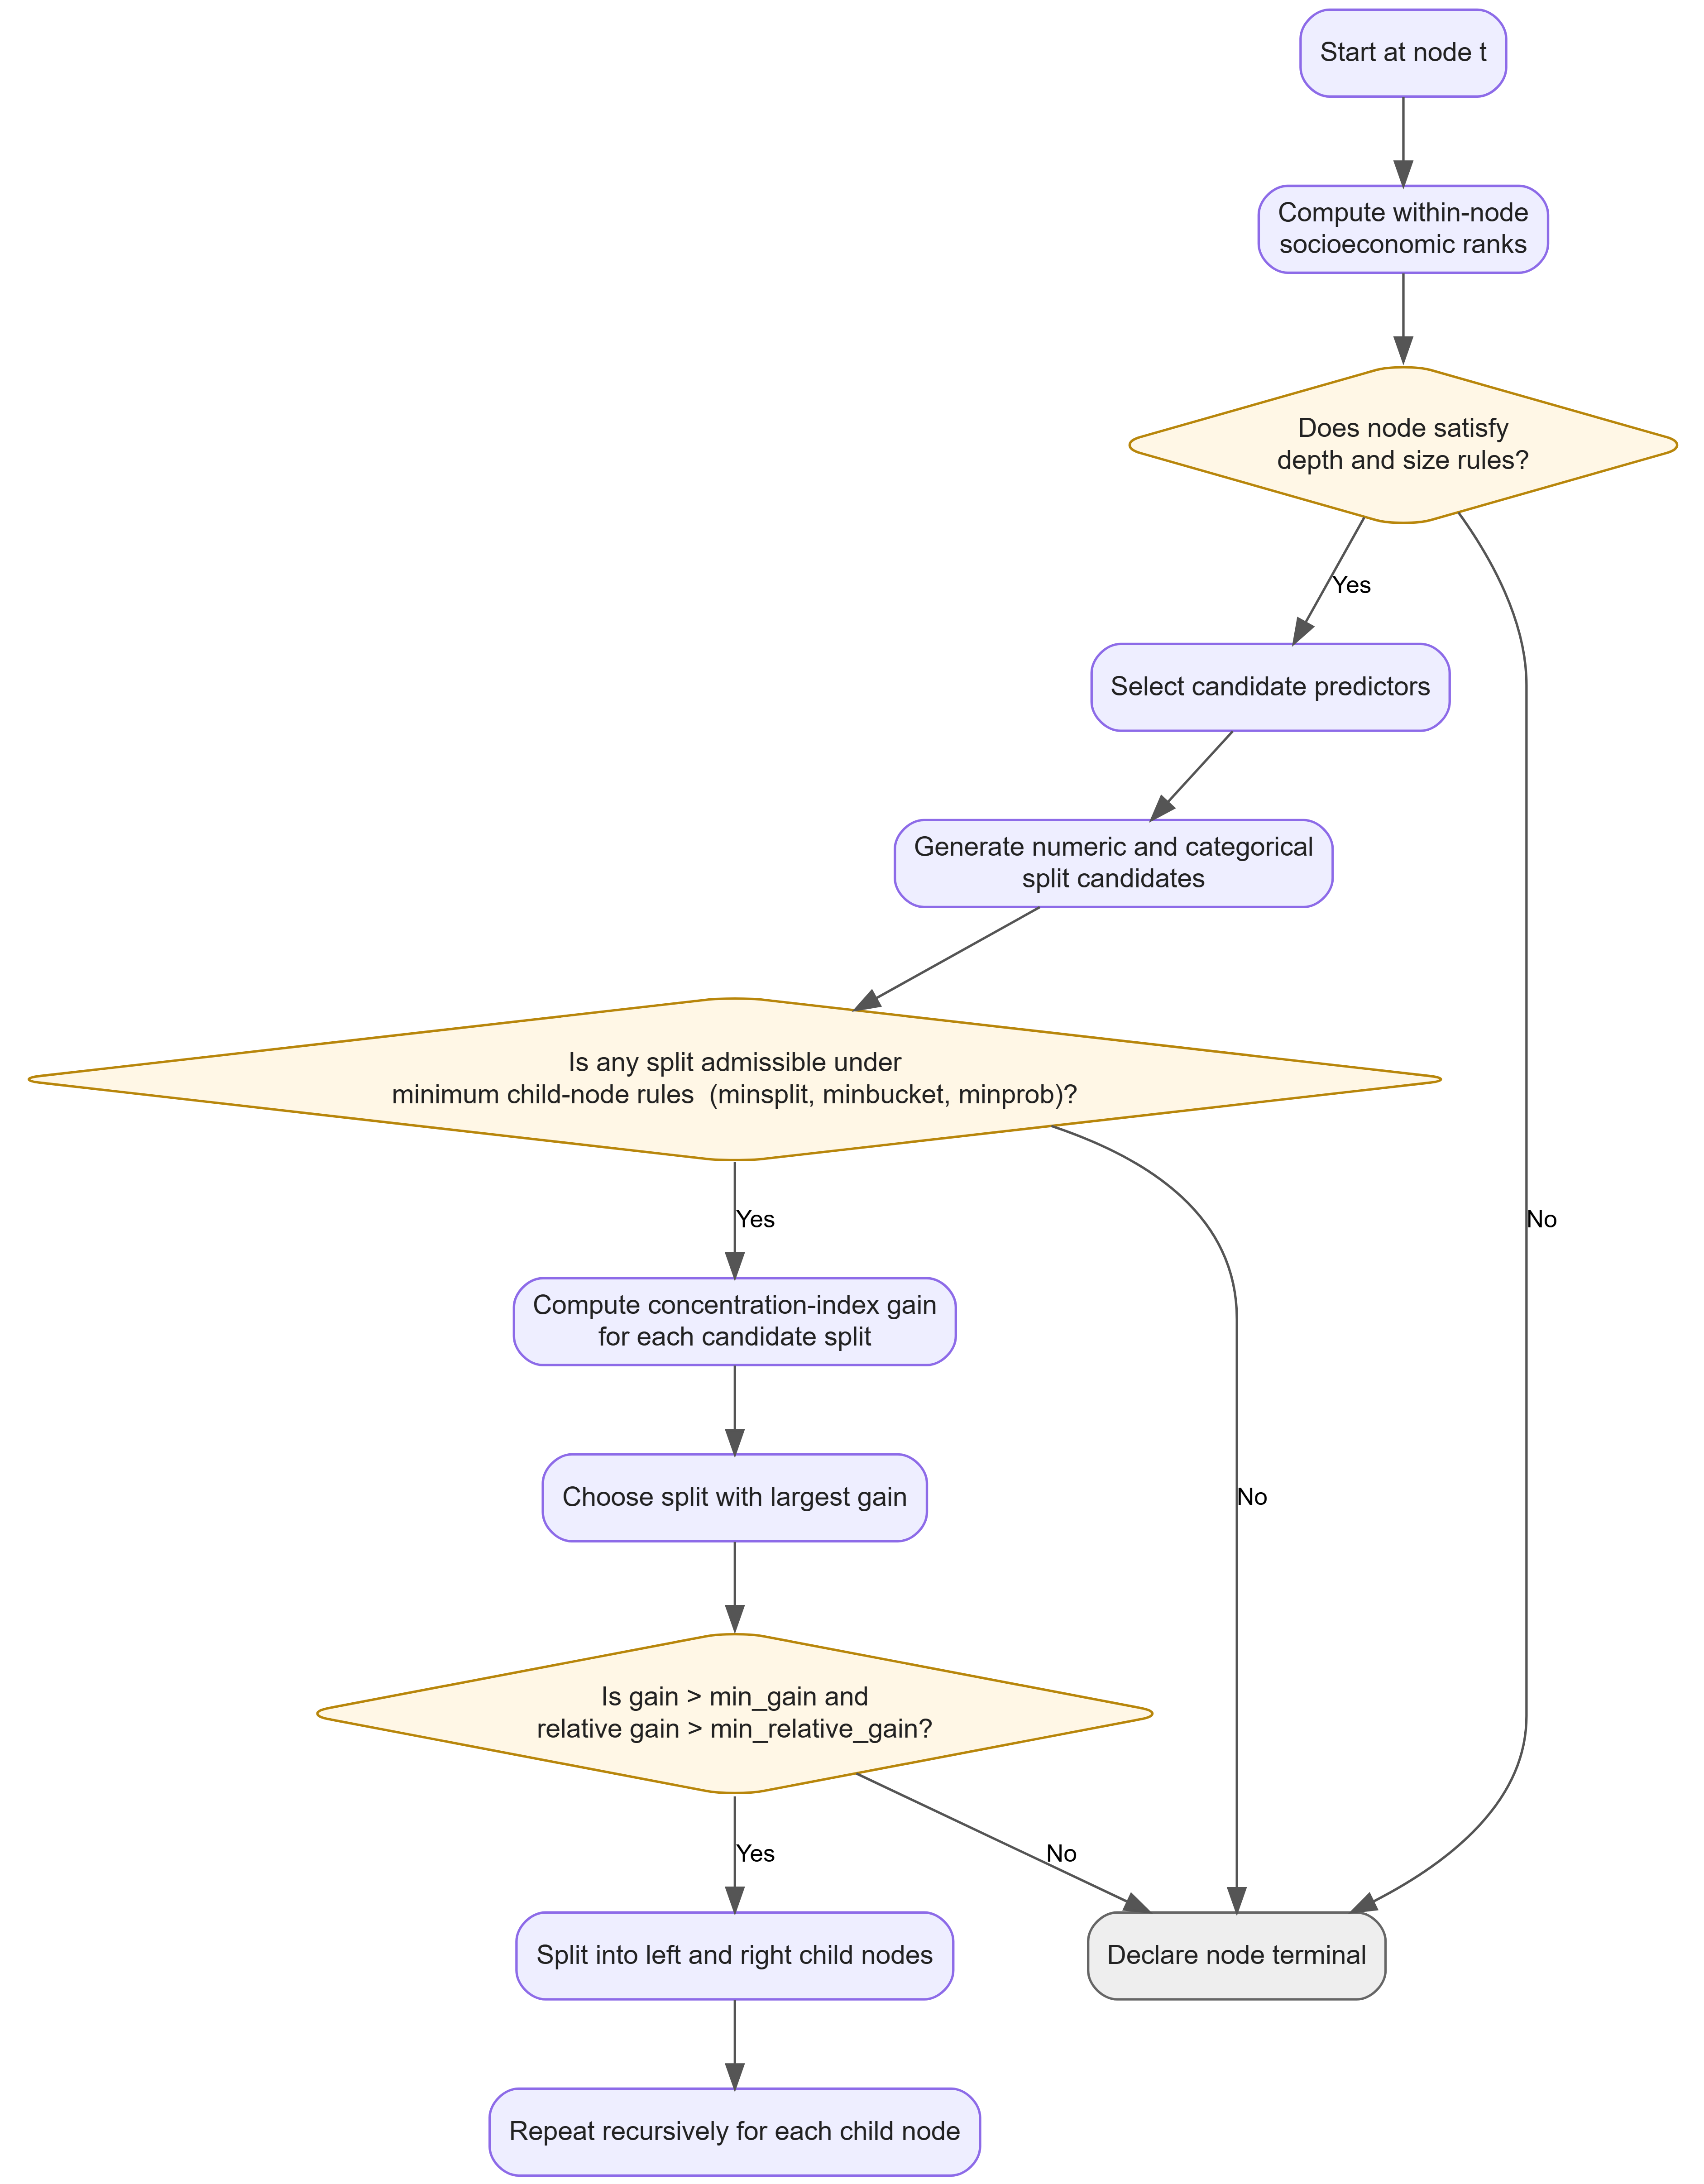
\includegraphics[width=5.5in,height=7in]{methodology_files/figure-latex/dot-figure-1.png}

}

\caption{\label{fig-greedy-ci-tree-flow}Greedy concentration-index
tree-growing procedure.}

\end{figure}%




\end{document}
